\subsection{Hydrodynamics and Collective Flow}
\label{Sec:Flow}

The initial discovery of strong elliptic flow at RHIC~\cite{Ackermann:2000tr} 
and the characteristic hydrodynamic signature of mass ordering 
in the medium response~\cite{Adler:2003kt,Kolb:2003dz} focussed a great deal 
of attention on improving the relativistic hydrodynamic description 
of the quark-gluon plasma. (See Ref.~\cite{Gale:2013da} for a recent review.)
One of the most important recent discoveries made in heavy ion collisions since the last Long-Range Plan
is the persistence of density fluctuations from the initial state. 
Recent work~\cite{Mishra:2007tw,Voloshin:2003ud,Takahashi:2009na,Sorensen:2010zq,Alver:2010gr,Qiu:2011iv,ALICE:2011ab,Adare:2011tg,ATLAS:2012at,Adamczyk:2013waa}
demonstrates that these fluctuations survive through the expansion of the fireball and appear as correlations between produced particles.
Most previous approaches had approximated the incoming nuclei as smooth spheres and the initial overlap region as an ellipse. The survival of density and geometry fluctuations was first hinted at in measurements of cumulants related to the shape of the elliptic flow distribution~\cite{Adler:2002pu,Miller:2003kd}. The picture started to become more clear after measurements were made in Cu+Cu collisions where the relative fluctuations were more prominent in the smaller system~\cite{Alver:2008zza}.  Ultimately, a new paradigm emerged as the structure of the initial state was found to play a central role 
in determining the azimuthal anisotropies with respect to the event plane angles $\Phi_n$, parameterized in terms of transverse momentum $p_T$ and azimuthal angle $\phi$ as
\begin{equation}
\label{Eq:vnDef}
\frac{d^2n}{p_T dp_T d\phi}
\sim
1 
+ 2 v_2(p_T) \cos 2 (\phi - \Phi_2)
+ 2 v_3(p_T) \cos 3 (\phi - \Phi_3)
+ 2 v_4(p_T) \cos 4 (\phi - \Phi_4)
+ \dots
\end{equation}
Previous measurements that were focused almost exclusively on the dominant $v_2$ were generalized to $v_n$, a spectrum carrying information about both the initial densities in the collision and the dissipative properties of the subsequent plasma phase~\cite{Heinz:2013th}. The survival of the initial state fluctuations is related to the earlier finding that the QGP discovered at RHIC is the most perfect fluid known~\cite{Teaney:2003kp,Romatschke:2007mq,Song:2010mg} with a viscosity to entropy ratio near the string theory limit~\cite{Kovtun:2004de}. 
The low viscosity plasma phase acts as a lens (albeit of strongly non-linear character), faithfully transferring the geometric structure of the initial density distributions, with its associated distribution of pressure gradients which act as a hydrodynamic force, into the final state. There it shows up most prominently as correlations between produced particles. Quantum fluctuations in the initial state cause these correlations to fluctuate from event to event.

Descriptions of these new phenomena have required the development of a new dynamical framework for heavy-ion collisions. It includes i) modeling of initial-state quantum fluctuations of nucleon positions and sub-nucleonic color charges and the color fields generated by them, ii) a description of the pre-equilibrium dynamics that evolves the initial energy-momentum tensor by solving either the (2+1)-dimensional Yang-Mills equations for the gluon fields (weakly-coupled approach) or Einstein's equations of motion in five-dimensional anti-deSitter space (strongly-coupled approach), followed by iii) the rapid transition, event-by-event, to second-order viscous relativistic fluid dynamics, and iv) a late-stage hadron phase described by microscopic transport calculations. 
While there is widespread agreement on the general structure of such a standardized dynamical approach, it has not yet reached the level of uniqueness that would justify calling it the ``Little Bang Standard Model'' \cite{Heinz:2013wva}. 
Model comparisons with experimental data that illustrate the state of the art in dynamical modeling can be found in 
Refs.~\cite{Schenke:2010rr,Song:2010mg,Song:2010aq,Schenke:2011bn,Schenke:2012wb,Gale:2012rq,Song:2013tpa,Song:2013qma,vanderSchee:2013pia,Habich:2014jna}. With the existence of a reliable equation of state from lattice 
QCD calculations~\cite{Bazavov:2009zn,Borsanyi:2010cj,Borsanyi:2013bia,Bazavov:2014pvz} a crucial degree of uncertainty in hydrodynamic modeling could be eliminated, enabling the development of a complete hydrodynamic space-time model. With this full space-time picture in hand, the comparisons of model calculations to 
harmonic decompositions of correlation functions ($\sqrt{v_{n}^{2}}$) at RHIC and the LHC (shown in Figure~\ref{fig:vn}) have reduced the uncertainty on $\eta/s$ by a factor of 10~\cite{Gale:2013da}. With this newfound precision, studies suggest that $\eta/s$ is smaller for RHIC collisions (right panel of Figure~\ref{fig:vn}) than it is at the LHC (left panel), consistent with a temperature dependent $\eta/s$ with a minimum near the critical temperature. In the next phase of study we seek to 1) accurately determine the temperature dependence of $\eta/s$ (aided by the Beam Energy Scan Program at RHIC described
in Sections~\ref{Sec:BES},~\ref{Sec:FacilitiesFuture} and~\ref{Sec:CP}) and 2) develop a clearer picture of the high density gluon fields discussed in Section~\ref{Sec:Saturation} that form the precursor of the plasma phase (aided by the p+A program 
and ultimately by an Electron Ion Collider).

\begin{figure}[ht]
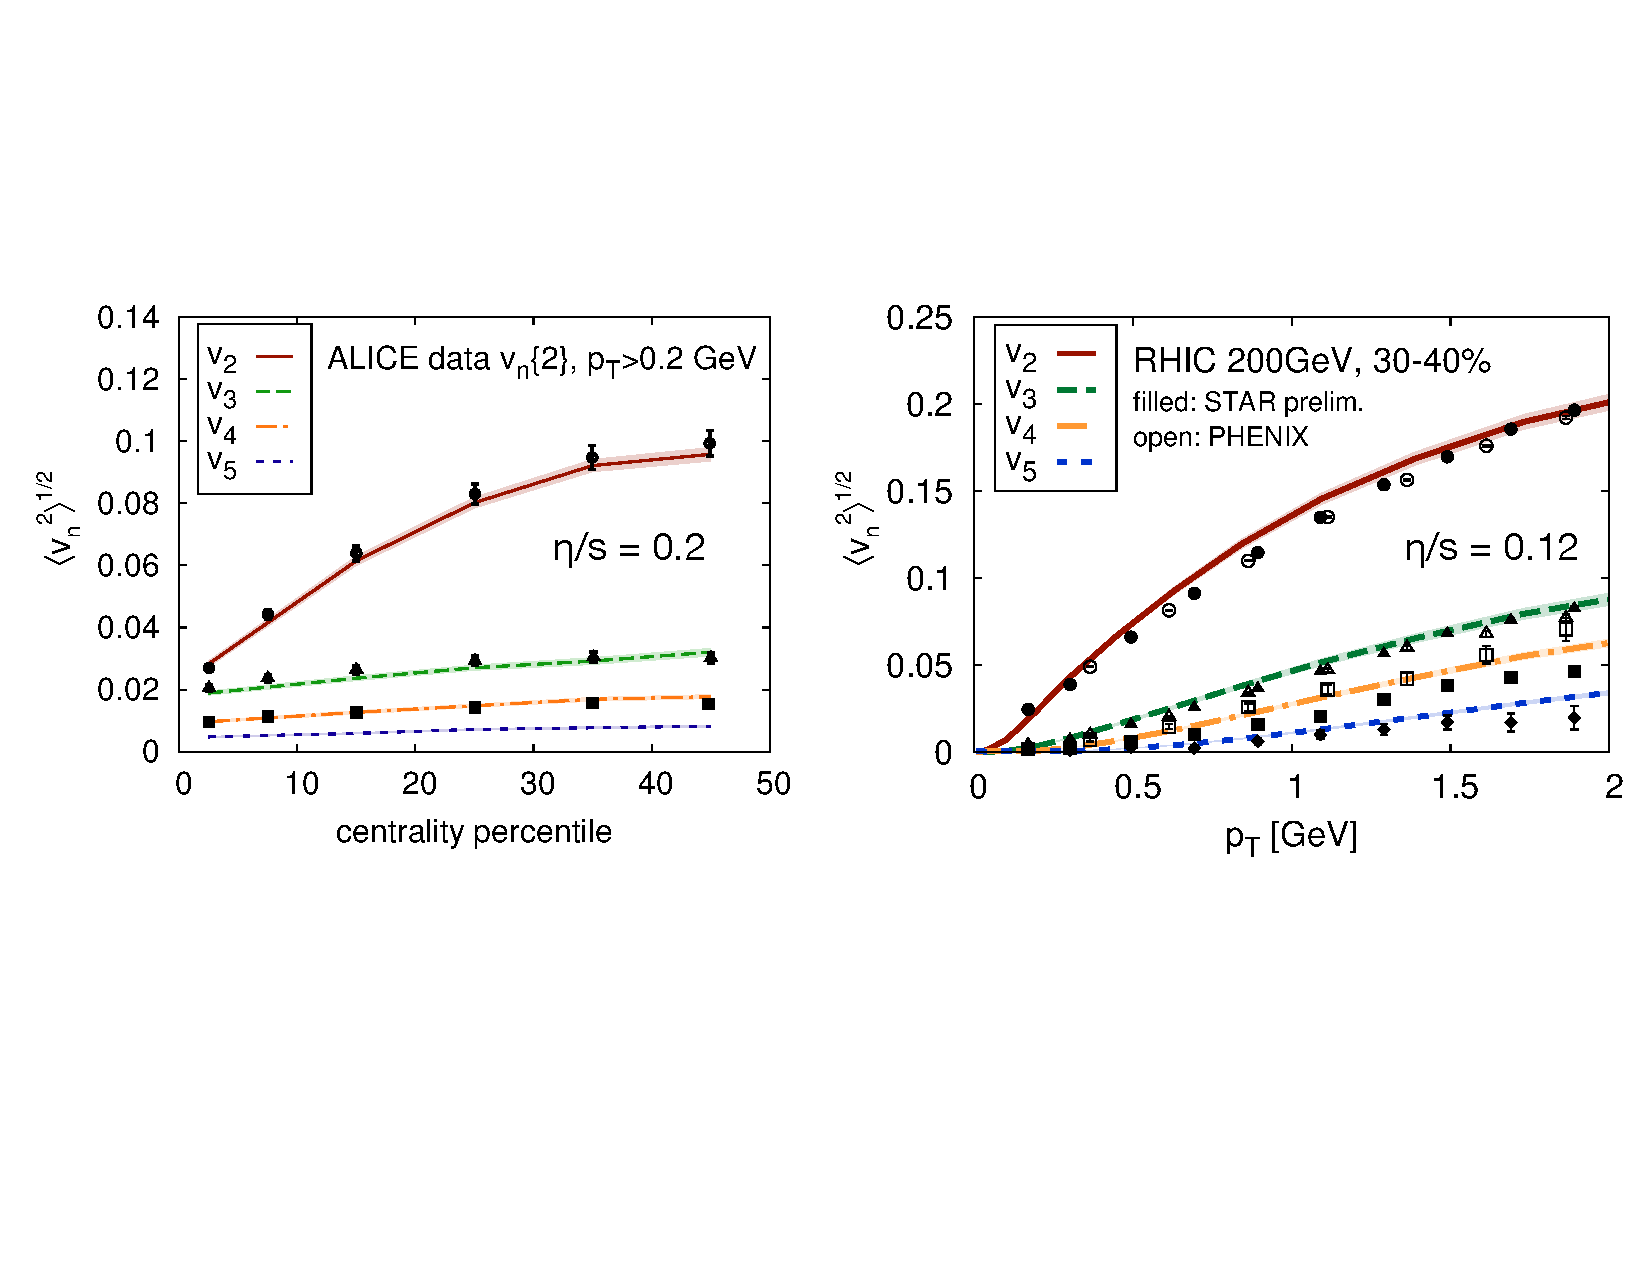
\includegraphics[width=1.\textwidth]{fig/RHIC_LHC_vn_calc.pdf}
\caption[Elliptic flow $v_2$ compared to a hydrodynamic model]{Model calculations compared to measurements of the harmonic decomposition of azimuthal correlations produced in heavy ion collisions~\cite{Gale:2013da}. The left panel shows model calculations and data for $v_n$ vs. collision centrality in Pb+Pb collisions at $\sqrt{s_{NN}}=2.76$ TeV. The right panel shows similar studies for the $p_T$ dependence of $v_n$ in 200 GeV Au+Au collisions. The comparison of the two energies provides insight on the temperature dependence of $\eta/s$. }
\label{fig:vn}
\end{figure}


What is needed to turn this standard dynamical framework into the ``Little Bang Standard Model''? One fundamental challenge along the way is the need to determine {\em simultaneously} the space-time picture of the collective expansion and the medium properties that drive this expansion~\cite{Heinz:2013wva}.
A unique and reliable determination of these two unknowns
will be informed by measurements of multiple flow observables sensitive to
medium properties in different stages of the evolution~\cite{Bhalerao:2011yg,Heinz:2013th,Jia:2014jca}. Due to the
large event-by-event fluctuations in the initial state collision
geometry, the matter created in each collision follows a different
collective expansion with its own set of flow harmonics (magnitude
$v_n$ and phases $\Phi_n$). Experimental observables describing
harmonic flow can be generally given by the joint probability
distribution of the magnitude $v_n$ and phases $\Phi_n$ of flow
harmonics:
\begin{equation}
\label{eq:flow1}
p(v_n,v_m,..., \Phi_n, \Phi_m, ...)=\frac{1}{N_{\mathrm{evts}}}\frac{dN_{\mathrm{evts}}}{dv_ndv_m...d\Phi_{n}d\Phi_{m}�}.
\end{equation}
Specific examples include the probability distribution of individual
harmonics $p(v_n)$, correlations of amplitudes or phases between different
harmonics ($p(v_n,v_m)$ or $p(\Phi_n,\Phi_m)$), and flow de-correlations in transverse and longitudinal
directions. These observables can be accessed through measurements of correlations with three or more
particles. 
The joint probability distribution (\ref{eq:flow1}) can be fully characterized experimentally by measuring the complete set of moments recently identified in Ref.~\cite{Bhalerao:2014xra}. 
With the added detail provided by these measurements,
hydrodynamic models can be fine-tuned and over-constrained, thereby
refining our understanding of the space-time picture and medium
properties of the QGP created in heavy ion collisions. Initial measurements of some
of these observables~\cite{Aad:2013xma,Aad:2014fla,GranierdeCassagnac:2014jha} and 
comparison to hydrodynamic and transport models~\cite{Gale:2012rq,Heinz:2013bua,Qiu:2012uy,Bhalerao:2013ina} 
have already provided unprecedented insights into the nature of the initial density
fluctuations and dynamics of the collective evolution, as seen in Figure~\ref{Fig:ebye}. 

\begin{figure}[hbt]
\begin{center}
\centerline{  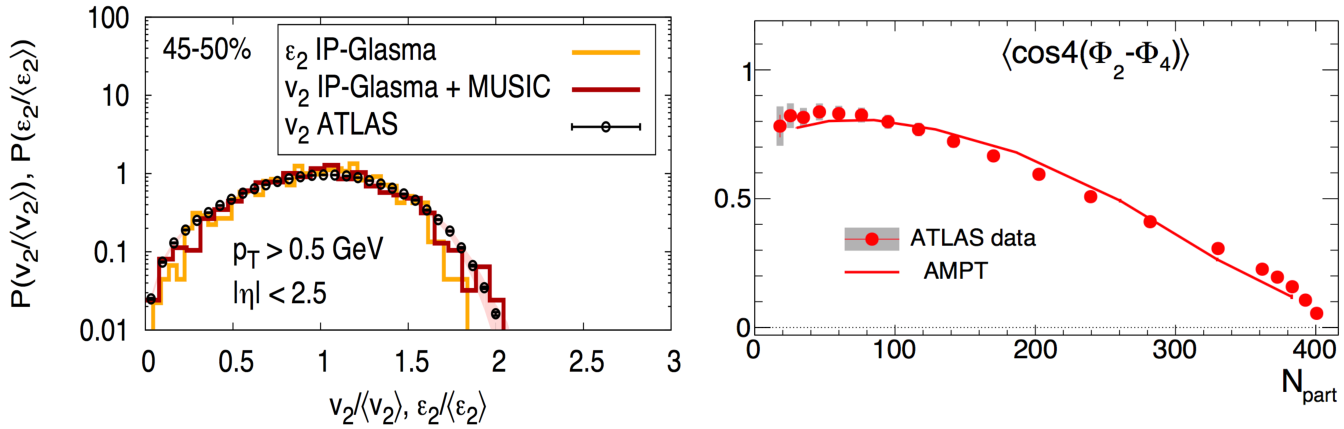
\includegraphics[width=1.0\textwidth]{fig/ebye.pdf}}
\caption[Hydrodynamic and transport models compared to flow observables]{Comparision of the $p(v_2)$ (left panel) and correlation between $\Phi_2$
  and $\Phi_4$ (right panel) measured for Pb+Pb collisions at
  $\sqrt{s_{NN}}=2.76$ TeV with hydrodynamic model~\cite{Gale:2012rq}
  or transport model~\cite{Bhalerao:2013ina} calculations.}
  \label{Fig:ebye}
\end{center}
\end{figure}


The agreement between the models and the data shown in
Figure~\ref{fig:vn} and Figure~\ref{Fig:ebye} suggests that the
essential features of the dynamic evolution of heavy ion collisions
are well described by our current models.  However, these model calculations
depend on the values assumed for many parameters, so reliable determination of the QGP
properties requires a systematic examination of the full parameter
space. An example of such an exploration~\cite{Novak:2013bqa} is shown
in Figure~\ref{fig:EOS} where the shape of the QCD equation of state (EOS) is treated as a
free parameter. 
he left panel shows a random sample of the thousands of possible Equations of State, constrained only by results on the velocity of sound obtained by perturbative QCD at asymptotically high temperature and by lattice QCD at the crossover transition temperature. They are compared to the EOS determined from lattice QCD \cite{Bazavov:2014pvz}.The right panel shows a sample of the Equations of State allowed by experimental data. The results of this study suggest that data at RHIC and the LHC require an EOS consistent with that expected from QCD. This demonstrates that our model of heavy-ion collisions describes the dynamics of the collisions well enough that we can extract information on the emergent properties of finite temperature QCD from the experimental traces left by the tiny droplet of QGP created in the collisions. These state-of-the-art models can therefore be used to both determine properties of finite temperature QCD currently inaccessible to lattice calculations and to provide an accurate space-time profile needed for modeling other processes like jet quenching. 
Figure~\ref{fig:visc}
shows a schematic representation of our current uncertainty on the
temperature dependence of $\eta/s$ in QCD matter. 
While many of the existing measurements are accurate enough, as seen in Figure~\ref{fig:vn}, to determine $\eta/s$ with much greater precision {\it if all other model parameters were already known}, the non-linear simultaneous dependence of the observables on multiple parameters does not yet allow one to translate the high quality of these experimental data into a more precise estimate of $\eta/s$.
The studies shown in
Figures~\ref{fig:vn}, \ref{Fig:ebye} and \ref{fig:EOS} 
suggest, however, that a more complete set of measurements of the moments of the joint probability distribution (\ref{eq:flow1}) at the LHC and RHIC (particularly in the Beam Energy Scan), coupled with extensive quantitative modeling, will provide the desired access to $(\eta/s)(T)$ in and around the transition temperature where hadrons melt into quark-gluon plasma, and strongly reduce the width of the blue uncertainty band in Figure~\ref{fig:visc}.




\begin{figure}[hbt]
\begin{center}
\centerline{  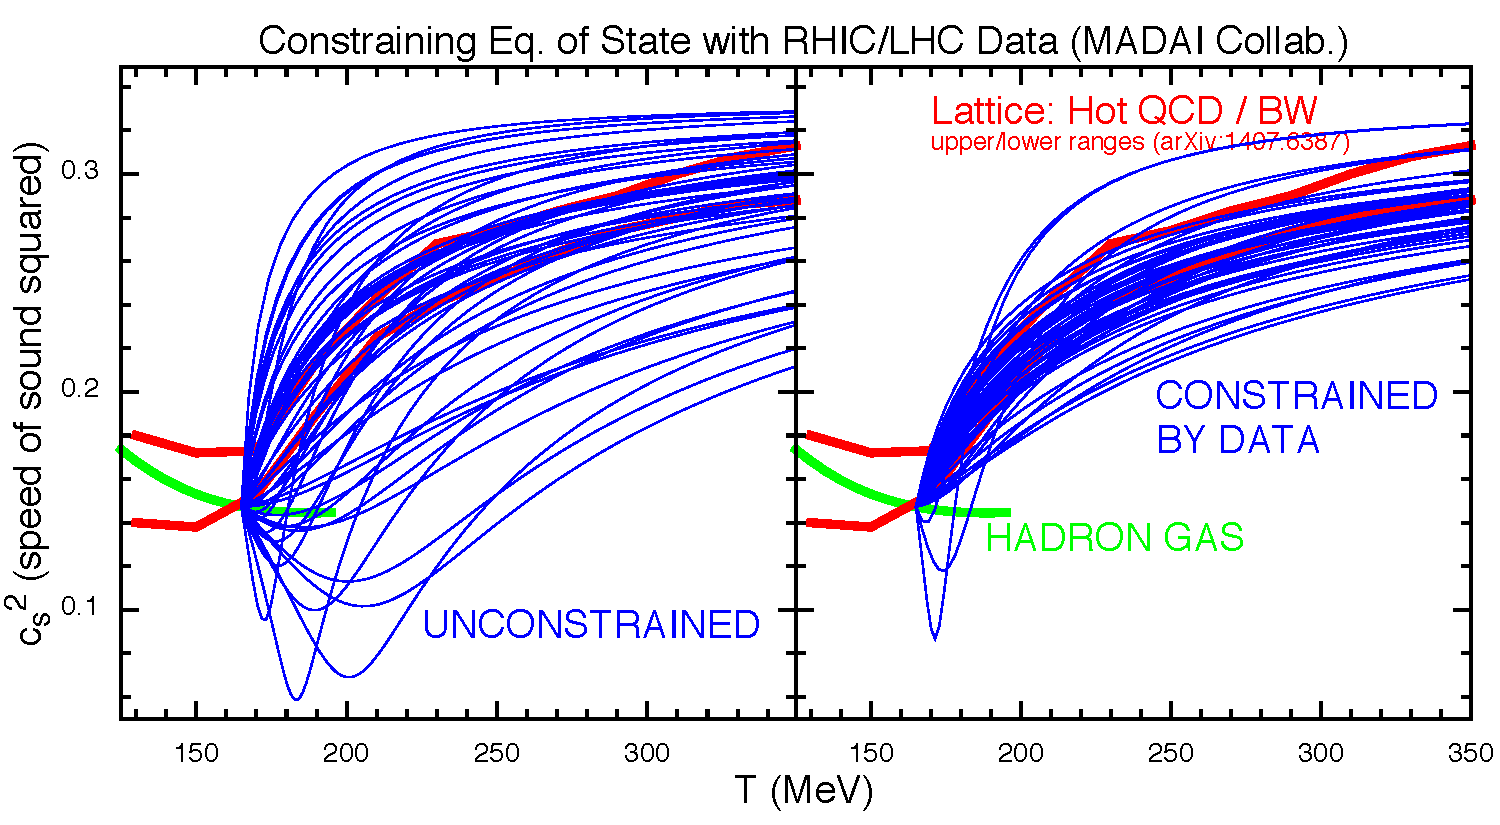
\includegraphics[width=.95\textwidth]{fig/priorvpost50.pdf}}
\caption[Constraints on the equation of state from RHIC and LHC data]{ Studies of the QCD equation of state from Lattice QCD calculations and from models constrained by data from RHIC and the LHC~\cite{Novak:2013bqa}. The right panel shows that data prefer an equation of state consistent with lattice QCD demonstrating that our model of the collision dynamics is good enough to allow us to study the emergent properties of QCD. }
  \label{fig:EOS}
\end{center}
\end{figure}


\begin{figure}[hbt]
\begin{center}
\centerline{  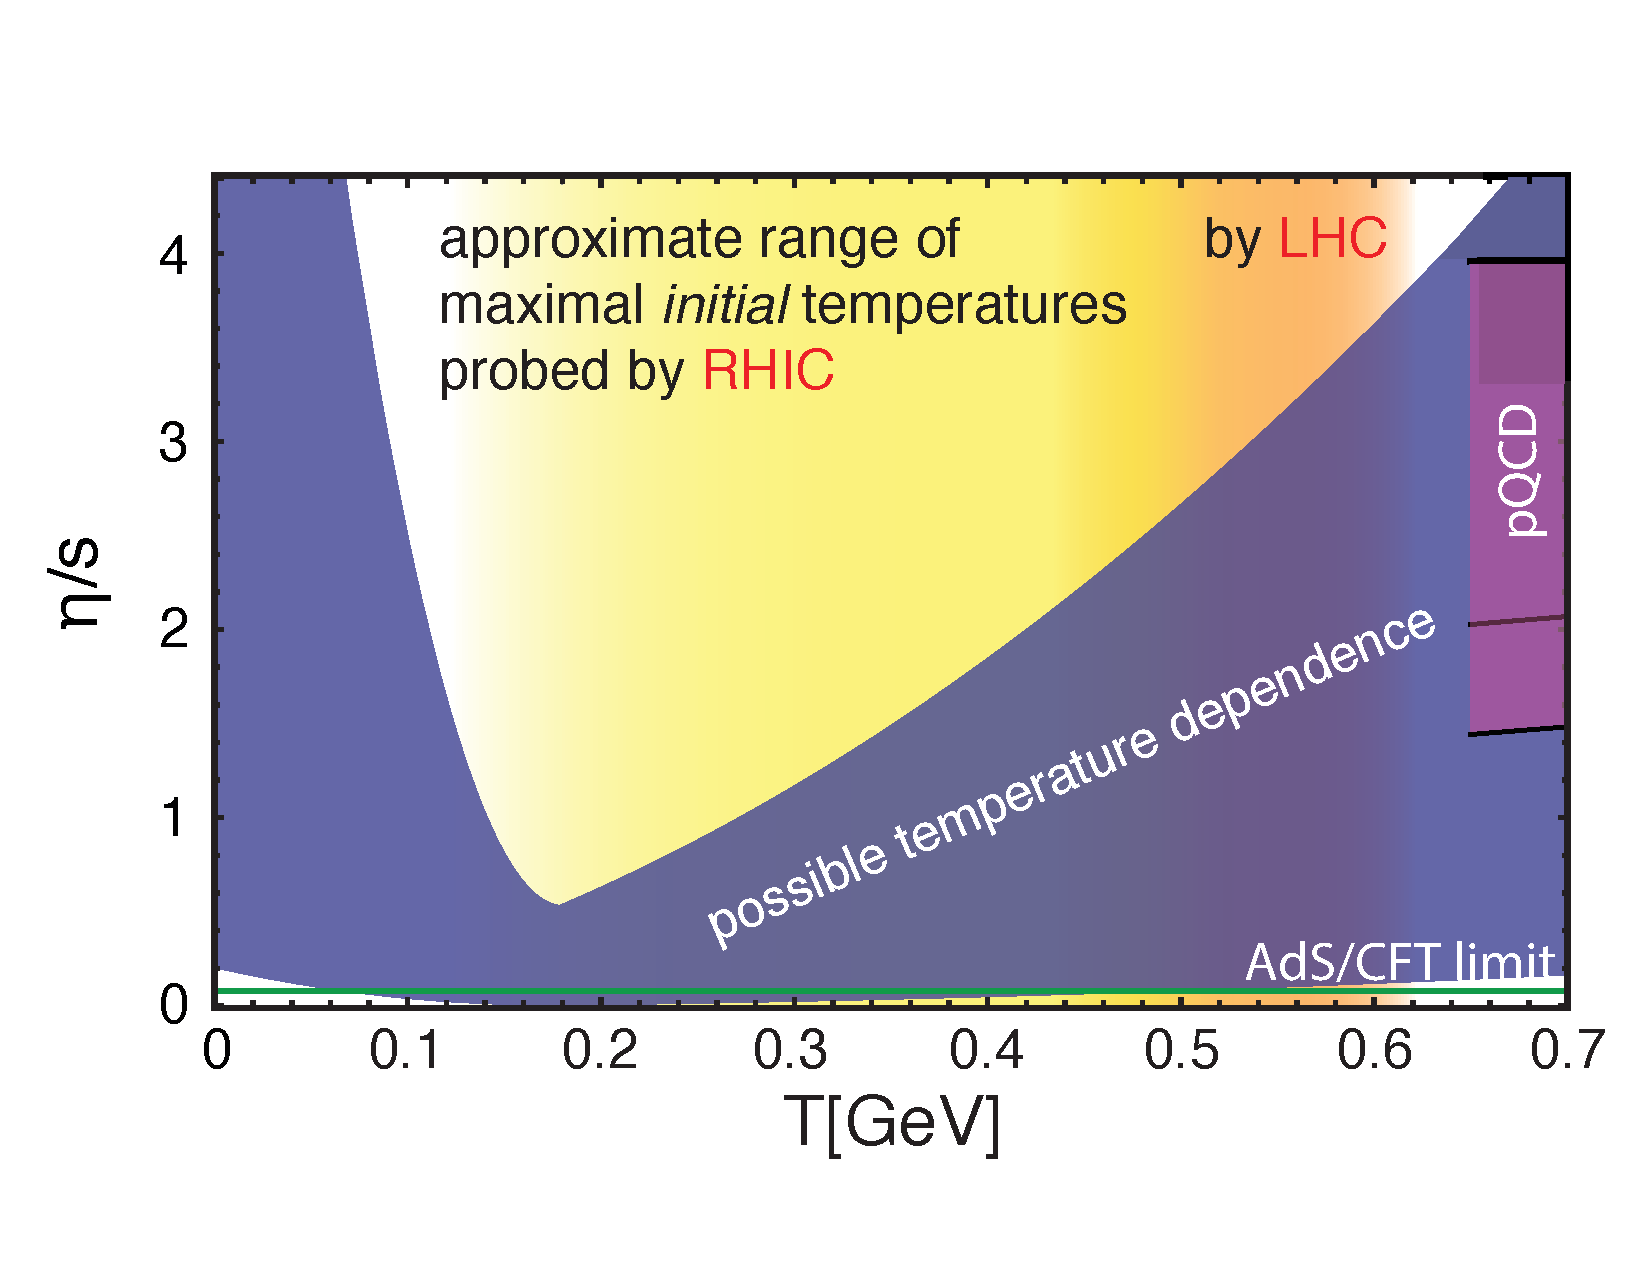
\includegraphics[width=.95\textwidth]{fig/visc_temp_dep.pdf}}
\caption[Temperature dependence of the viscosity to entropy density $\eta/s$]{The temperature dependence of the viscosity to entropy density $\eta/s$. The blue band represents the range allowed by our current understanding based on models compared to data with a minimum at the transition temperature. pQCD calculations and the string theory limit are also shown. The shaded vertical regions represent the ranges of initial temperatures probed by RHIC and the LHC.}
  \label{fig:visc}
\end{center}
\end{figure}

While the paradigm of collective flow phenomena in a strongly coupled,
opaque QGP fluid has been firmly established in sufficiently central
collisions of heavy nuclei, it was generally expected that the
magnitude of collectivity would diminish as the system size
decreases. As the mean-free-path of the matter approaches the
characteristic size of the system, the effects of viscous damping
become more important and the validity of a hydrodynamic description
becomes more suspect. Evidence for this trend has been observed in
peripheral A+A collisions. As such, no collective flow was anticipated
in \pp\ and \pA\ collisions. Surprisingly, 
correlations that are
long-range in rapidity and similar to those measured in A+A collisions
have now also been observed at the LHC in rare high-multiplicity
p+p collisions~\cite{Khachatryan:2010gv} (corresponding to high
gluon-density initial states). 
In several ways, these resemble the
correlations in central A+A collisions which have been widely accepted as
evidence of collective flow~\cite{Ollitrault:1992bk,Voloshin:1994mz}.
Subsequent measurements revealed similar phenomena in high
multiplicity \pPb\ and \dAu\ at both the
LHC~\cite{CMS:2012qk,Abelev:2012ola,Aad:2012gla} and
RHIC~\cite{Adare:2013piz}. The dependence of the correlations in
\pPb\ or \dAu\ on $p_T$,
multiplicity~\cite{Aad:2013fja,Chatrchyan:2013nka,Abelev:2014mda,Aad:2014lta},
pseudorapidity~\cite{CMS-PAS-HIN-14-008}, and particle
species~\cite{ABELEV:2013wsa,Khachatryan:2014jra} reveal similarities
to those observed in A+A collisions. In particular, the mass ordering
of $v_n(p_T)$ is reminiscent of the effect from a common radial flow
boost in A+A collisions~\cite{ABELEV:2013wsa,Adare:2014keg,Khachatryan:2014jra}, and
multi-particle correlations show unambiguously that the novel correlations in
high-multiplicity \pPb\ collisions are collective in
nature~\cite{GranierdeCassagnac:2014jha}.


The origin of collectivity in these small systems is a topic of
debate. While hydrodynamic models with strong final-state interactions
may provide a natural interpretation for many of the observed features
in the
data~\cite{Bozek:2009dt,Bozek:2011if,Bozek:2012gr,Schenke:2014zha,Werner:2013ipa},
their apparent applicability in such small systems, along with the required assumption of
rapid thermalization, challenges our understanding~\cite{Niemi:2014wta}. Meanwhile, other novel
mechanisms, mainly related to the initial-state quark and gluon
correlations, have also been proposed as alternative interpretations of the
observed long-range correlations in \pA\ and \dA\ collisions, 
and they have even provided qualitatively successful descriptions for \pp\
collisions~\cite{Dumitru:2010iy,Dusling:2012cg,Dusling:2013oia,Gyulassy:2014cfa,Dumitru:2014yza}. Disentangling
initial- and final-state effects to distinguish between these various approaches poses a theoretical and experimental
challenge. Recent data from $^3$He+Au collision may shed some light on
the question, as will improved correlation measurements at forward
rapidity, where the presence of the correlation structures is
most surprising. 
Further insights are expected as
comprehensive studies of the system-size and geometric dependence
become available in \pA\, \dA\ and $^3$He+A
collisions~\cite{Nagle:2013lja} where the relative contributions of
initial- and final-state correlations are expected to vary. 
This program will allow us to explore the boundary of perfect
fluidity in QCD matter at the smallest scales ever
achieved~\cite{Shuryak:2013ke}. 

Addressing these open questions on the possible role of hydrodynamics
in the smallest hadronic systems will play an
important role not only in completing our standard model of a strongly
coupled QGP matter, but also in providing new opportunities to probe
the structure of protons. 
If indeed
final-state effects described by hydrodynamic flows are proven to be
the dominant source of correlations, the presence of a tiny low viscosity
fluid enables the study of protons and sub-nucleonic scale
fluctuations at very short time
scales~\cite{Coleman-Smith:2013rla,Schenke:2014zha,Schlichting:2014ipa}. 
The high-density gluon state inside a
proton is of fundamental interest as the equations of QCD are expected
to become classical~\cite{McLerran:1993ni,Gelis:2010nm}. This
transition has the potential to reveal how a classical system can emerge from
QCD. In light of recent exciting observations, this topic should be
studied in future \pA\ programs covering the wide kinematic range
provided by RHIC and the LHC and ultimately in an EIC which is the
highest priority for new construction in our community.

